%!TEX root = main.tex

\newpage
\appendix
\begin{landscape}

\global\pdfpageattr\expandafter{\the\pdfpageattr/Rotate 90}

\section{Appendix A - Gantt diagrams} \label{App:A}

\begin{figure}[!ht]  
\begin{center}  
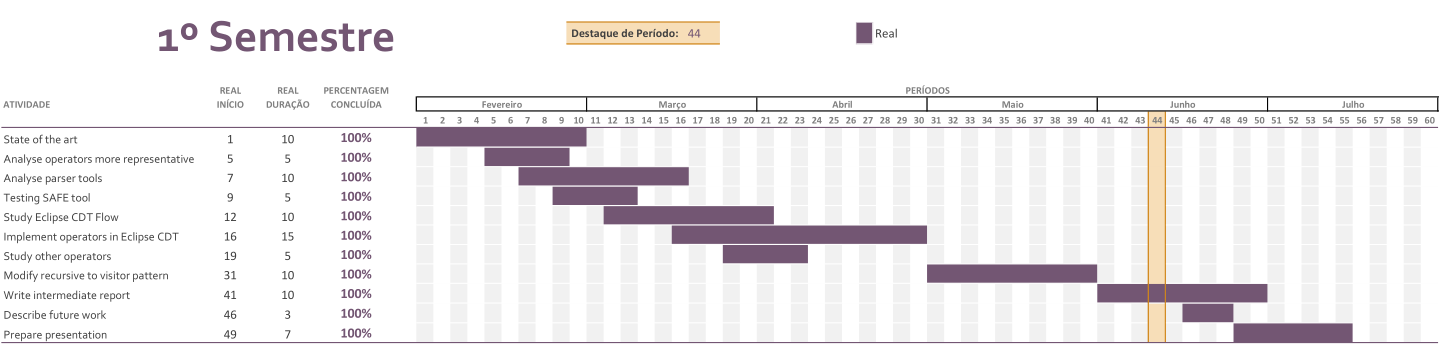
\includegraphics[width=1.6\textwidth]{img/gantt1.png}  
\caption{\small \sl Gantt first semester.\label{fig:gantt1}}  
\end{center}  
\end{figure}

\begin{figure}[!ht]  
\begin{center}  
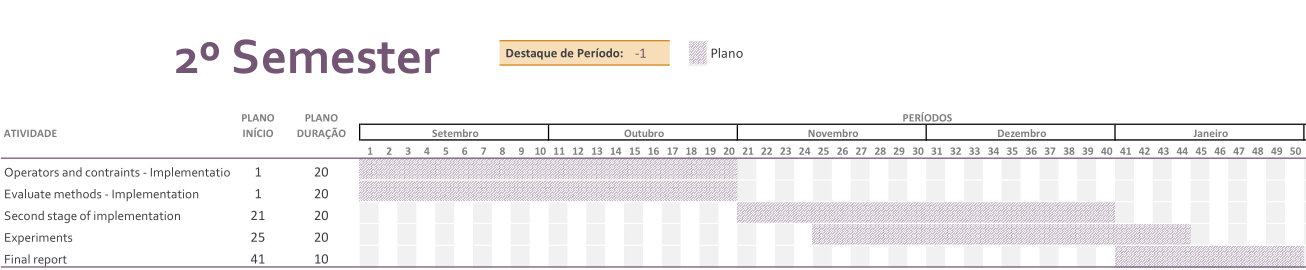
\includegraphics[width=1.6\textwidth]{img/gantt2.png}  
\caption{\small \sl Gantt seconf semester.\label{fig:gantt2}}  
\end{center}  
\end{figure}

\clearpage

\section{Appendix B - Risks table} \label{App:B}
\begin{figure}[!ht]  
\begin{center}  
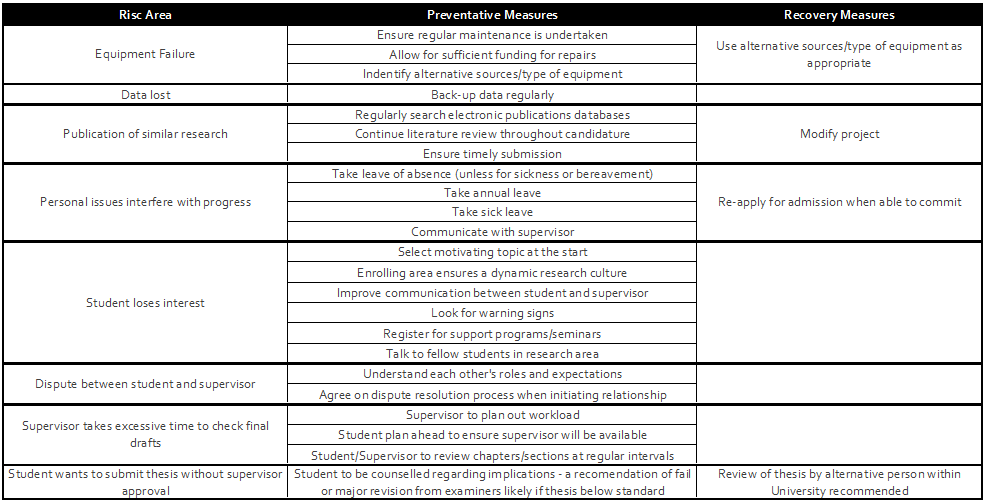
\includegraphics[width=1.5\textwidth]{img/risks.png}  
\caption{\small \sl Risks.\label{fig:risks}}  
\end{center}  
\end{figure}

%\newpage
%\section{Appendix B} \label{App:B}
%% the \\ insures the section title is centered below the phrase: Appendix B
%Text of Appendix B is Here


\end{landscape}
\global\pdfpageattr\expandafter{\the\pdfpageattr/Rotate 0}

\newpage
